% ***************************** MAIN FILE **********************************

\documentclass[12pt]{scrreprt}           % Art des zu erstellenden Dokuments
% bei zweiseitigem Druck twoside-Option oder book-Klasse verwenden

% ****************************** PREAMBLE **********************************
% **************************** PACKAGE SETUP *******************************
\usepackage[ngerman]{babel}          % Lokalisierung von Typographie, Silbentrennung, etc.

\usepackage{ucs}                     % Erweiterte Unterstützung von UTF-8-Kodierung
\usepackage[utf8x]{inputenc}         % Unterstützung von UTF-8 in Eingabe-Dateien
\usepackage[T1]{fontenc}             % Zeichensatzkodierung von LaTeX (Cork-Kodierung)
\usepackage{helvet,courier,mathptmx} % Verwendete Schriftarten

\usepackage[headsepline, plainheadsepline, plainfootsepline] {scrpage2}

\usepackage{amsmath}                 % Mathematische Infrastruktur für LaTeX der AMS
\usepackage{amsfonts}                % Mathematische Schriftarten
\usepackage{amssymb}                 % Mathematische Symbole
\usepackage{amsthm}                  % Erweiterung der Theorem-Umgebungen
\usepackage[]{units}					 % für \unit-Befehl
%\usepackage[amssymb]{siunits}		 % für SI-Einheiten (amssymb definiert den Befehl \square des amssymb Packages um. Ist dies nicht gewünscht kann die Option squaren verwendet werden. Dann muss für die SI-Einheiten \squaren anstatt \square verwendet werden.)

%\usepackage{fancyhdr}                % Erweiterte Konfiguration von Kopf/Fußzeile
\usepackage{hyperref}                % Querverweise, Hyperlink, pdf-Konfiguration, etc.

\usepackage{float}                   % Selbstdefinierte Floating-Umbgebungen
\usepackage{tabularx}                % Tabellen mit einstellbarer Spaltenbreite
\usepackage[labelfont=bf]{caption}   % Anpassen der Abbildungs- und Tabellenbeschriftungen

\usepackage{algpseudocode}           % Algorithmen als Pseudocode (basiert auf algorithmicx)
\usepackage{listings}                % Quellcode-Satz (z.B. mit Syntax-Hervorhebung)

\usepackage[pdftex,
%draft							%Figures werden nur als Platzhalter eingeblendet
]{graphicx}						% Erweiterte Unterstützung von Graphiken
\usepackage{textpos}                 % Beliebig platzierte Textboxen
\usepackage{xcolor}                  % TeX-Engine-unabhängige Definition von Farben
\usepackage[printonlyused]{acronym}


\usepackage{pdfpages}

\usepackage[numbers]{natbib}         % Weiter Optionen für die Bibliographie
\bibliographystyle{IEEEtranN}
\usepackage{todonotes}
\usepackage{tabulary}

% ****************************** TOP MATTER ***********************************
\renewcommand{\author}{Author}           % Name
\newcommand{\dateOfBirth}{Date}           % Geburtsdatum
\newcommand{\matrNumber}{matnr}              % Matrikelnummer
\newcommand{\studycourse}{Informatik}           % Studiengang

\newcommand{\supervisor}{Prof. Dr. Claus Fühner} % Betreuer
\newcommand{\institution}{Ostfalia Hochschule} % Hochschule
\newcommand{\subinstitution}{Hochschule Braunschweig/Wolfenbüttel}
\newcommand{\faculty}{Informatik}               % Fachbereich
\newcommand{\toponym}{Wolfenbüttel}                 % Ort

\renewcommand{\subject}{Seminararbeit}  % Art/Thema der Arbeit
\newcommand{\titel}{Titel der Arbeit} % Titel der Arbeit
\newcommand{\subtitel}{Untertitel} % Untertitel
\newcommand{\graduation}{} % Angestrebter Titel (nur bei Abschlussarbeiten, sonst leer lassen/auskommentieren)

\newcommand{\keywords}{{}} % Stichworte (durch Komma getrennt)


% **************************** HYPERREF SETUP *******************************
\definecolor{linkcolor}{rgb}{1,0.5,0}
\hypersetup
{
bookmarks=true,                        % Lesezeichen im PDF erzeugen
bookmarksopen=true,                    % Lesezeichen im PDF sofort anzeigen
backref=true,                          % Rückverweise im Literaturverzeichnis
colorlinks=true,                       % Farbige Verweise
%hidelinks = true,                      % Verweise verbergen (entfernt Farbe und Rahmen)
pdfstartview={FitH},                   % Ansicht des PDFs beim öffnen
pdftitle={\titel},                     % Title des PDFs
pdfauthor={\author , \supervisor},     % Autor des PDFs
pdfsubject={\subject},                 % Thema des PDFs
%pdfcreator={Creator},                 % Erzeuger des Dokuments (Anwendungsprogramm)
%pdfproducer={Producer},               % Ersteller des PDFs (Programm/Bibliothek/Skript)
pdfkeywords={\keywords},               % Stichwörter zum PDF
linkcolor=linkcolor,                   % Farbe von Querverweisen
citecolor=green,                       % Farbe von Zitaten
filecolor=magenta,                     % Farbe von Verweisen auf Dateien
urlcolor=cyan                          % Farbe von URLs
}
% Weitere Optionen: http://www.tug.org/applications/hyperref/manual.html

% **************************** LISTINGS SETUP *******************************
\definecolor{keywords}{rgb}{0.5 0 0.3}
\definecolor{comments}{rgb}{0.25,0.5,0.37}
\lstset{ %
  backgroundcolor=\color{white},   % Hintergrundfarbe
  basicstyle=\linespread{0.94}\footnotesize\ttfamily, % Schrifteinstellungen für Quellcode
  breakatwhitespace=false,         % Automatische Zeilenumbrüche nur bei Leer- oder Tabulatorzeichen (Leerraum/whitespaces)
  breaklines=true,                 % Automatische Zeilenumbrüche
  captionpos=b,                    % Beschriftung unten
  commentstyle=\color{comments},   % Schrifteinstellungen für Kommentare
%  deletekeywords={...},            % Bestimmte Schlüsselwörter entfernen
  escapeinside={\%*}{*)},          % Defintion von Escape-Sequenzen
  extendedchars=true,              % Nicht ASCII-Zeichen erlauben
  frame=single,                    % Rahmen um den Quellcode
  keepspaces=true,                 % Einrückungen im Quellcode behalten
  keywordstyle=\bfseries\color{keywords},% Schrifteinstellungen für Schlüsselwörter
  language=java,                   % Programmiersprache des Quellcodes
%  morekeywords={*,...},            % Zusätzliche Schlüsselwörter
  numbers=left,                    % Zeilennummerierung
  numbersep=5pt,                   % Abstand zwischen Zeilennummerierung und Quellcode
  numberstyle=\tiny\color{gray}, % Schrifteinstellungen für Zeilennummern
  rulecolor=\color{black},         % if not set, the frame-color may be changed on line-breaks within not-black text (e.g. comments (green here))
  showspaces=false,                % Leerraum-Zeichen anzeigen
  showstringspaces=false,          % Leerzeichen in Zeichenketten anzeigen
  showtabs=false,                  % Tabulatorzeichen in Zeichenketten anzeigen
  stepnumber=1,                    % Schrittweite bei Zeilennummern
  stringstyle=\color{blue},        % Schrifteinstellungen für Zeichenketten
  tabsize=4,                       % Tabulatorbreite (Anzahl Leerzeichen)
  numberbychapter=false            % Nummeriere Quellcode fortlaufend je Kapitel
}
\renewcommand{\lstlistlistingname}{Quellcodeverzeichnis}
\renewcommand{\lstlistingname}{Quellcode}

\AtBeginDocument{\numberwithin{lstlisting}{section}} % Nummeriere Quellcode fortlaufend je Abschnitt

% ************************** HEADER/FOOTER SETUP ****************************
\pagestyle{scrheadings}

\clearscrheadings				% löscht voreingestellte Stile
\clearscrplain					% löscht voreingestellte Stile

\lohead[\headmark]{\headmark}
\rohead[\pagemark]{\pagemark}

\automark{chapter}

% **************************** GRAPHICX SETUP *********************************
\DeclareGraphicsExtensions{.pdf,.png,.jpg} % bekannte Graphik-Dateiformate (müssen nicht mehr im Dateinamen angegeben werden, also statt "beispiel.png" nur noch "beispiel")
\graphicspath{{./figure/}}   % path to graphics folder, usage {PATH},{ANOTHERPATH}...

% ************************** BIBLIOGRAPHY SETUP ********************************
%\bibliographystyle{alphadin}    % Literaturverzeichnis nach DIN
%\AtBeginDocument{\nocite{*}} % Diese Zeile vor der Abgabe der Arbeit entfernen!

% ****************************** MATH SETUP ************************************
\everymath{\displaystyle}    % Erzwinge \displaystyle für Mathematischen-Modus


% ************************* THEOREMS AND PROOF *********************************
\newtheoremstyle{thesis}     % Name des neuen Theorem-Stils
{3pt}                        % Abstand oberhalb des Theorems
{3pt}                        % Abstand unterhalb des Theorems
{\itshape}                   % Schrifteinstellungen innerhalb des Theorems
{}                           % Einrückung der Theorem-Überschrift
{\bfseries}                  % Schrifteinstellungen für die Überschrift des Theorems
{}                           % Satzzeichen zwischen Überschrift und Theorem-Rumpf
{\newline}                   % Abstand hinter der Überschrift
{}                           % Spezifikation der Überschrift
  
\theoremstyle{thesis}        % Verwende neuen Theorem-Stil

\newtheorem{theorem}{Satz}[section] % neue Theorem-Umgebung: theorem (Satz)
\providecommand*{\theoremautorefname}{Satz} % autoref-Name für theorem

\newtheorem{definition}{Definition}[section] % neue Theorem-Umgebung: definition (Definition)
\providecommand*{\definitionautorefname}{Definition} % autoref-Name für definition

\renewcommand{\qedsymbol}{$\blacksquare$} % Schwarzes Quardrat als Symbol für: q. e. d.
\renewenvironment{proof}[1][\proofname]{{\bfseries #1:}~}{\qed} % "Beweise:" in Fettdruck

% *************************** PSEUDOCODE SETUP ********************************
\floatstyle{boxed}                        % Rahmen für pseudocode-Umgebung
\newfloat{pseudocode}{htbp}{lop}[section] % Definieren pseudocode-Umgebung
\floatname{pseudocode}{Pseudocode}        % Beschrifte pseudocode-Umgebung mit "Pseudocode"

\newcommand{\listofpseudocodename}{Pseudocodeverzeichnis}
\newcommand{\listofpseudocode}{\listof{pseudocode}{\listofpseudocodename}}
\providecommand*{\pseudocodeautorefname}{Pseudocode}

% ******************************* PAGE SETUP **********************************
\textheight23cm
\textwidth14cm
\voffset0cm
\topskip0cm
\topmargin-1.2cm
\headheight1.0cm
\headsep1.5cm
\oddsidemargin1.0cm
\evensidemargin1.0cm
\renewcommand{\baselinestretch}{1.4} 

% Hurenkinder und Schusterjungen verhindern
\clubpenalty = 10000
\widowpenalty = 10000
\displaywidowpenalty = 10000

% Verbesserung der Textsetzung
\tolerance = 1000
\emergencystretch = 20pt

% ******************************** MACROS *************************************
\newcommand{\RR}{\mathbf{R}}
\newcommand{\NN}{\mathbf{N}}
\newcommand{\QQ}{\mathbf{Q}}
\newcommand{\ZZ}{\mathbf{Z}}
\newcommand{\CC}{\mathbf{C}}


%%%%%%%%%%%%%%%%%%%%%%%%%%%%%%%%%%%%%%%%%%%%%%%%%%%%%%%%%%%%%%%%%%%%%%%%%%%%%%%
% ************************** BEGINN OF DOCUMENT *******************************
%%%%%%%%%%%%%%%%%%%%%%%%%%%%%%%%%%%%%%%%%%%%%%%%%%%%%%%%%%%%%%%%%%%%%%%%%%%%%%%
\begin{document}

\pagestyle{plain}

% 
%% *** Titelseite ***
%
\begin{titlepage}
	\vspace*{-3.0cm}
	%Logo international
	%\hspace*{ 9.30cm}
\includegraphics[scale=0.93]{../ostfalia/LSVorlagejpg_klein_int.jpg}\\
	%Logo deutsch
	%\hspace*{10.20cm}
\includegraphics[scale=0.60]{../ostfalia/Ostfalia_LS_RGB_klein.jpg}\\
	\hspace*{ 6.90cm}
\includegraphics[scale=0.93]{../ostfalia/Ostfalia_LS_RGB_klein.jpg}\\
	%Logo ohne Schrift
	%\hspace*{15.00cm}
\includegraphics[scale=0.60]{../ostfalia/Ostfalia_L_RGB_klein.jpg}\\
	%\hspace*{14.30cm}
\includegraphics[scale=0.93]{../ostfalia/Ostfalia_L_RGB_klein.jpg}\\
	\hspace*{-1.00cm}
\includegraphics[scale=1.20]{../ostfalia/Reiter_Wolfen_RGB_174mm.jpg}\\
	
	\hspace*{-0.5cm}{\Large\textsf{Fakultät \faculty}}\\
	
	\hrulefill\\
	
	%-------------------------------------------------------------------------------
	\begin{flushleft}
	{\Large\textsf{\authorMarco, \matrNumberMarco\\}}
	{\Large\textsf{\authorNiklas, \matrNumberNiklas\\}}
	\end{flushleft}
	
	
	
	
	\begin{center}
	\vspace{2em}
	\textbf{
	\textsf{\huge\titel \\[0.3ex]}}
	\textsf{\hspace*{0.5cm}\large \subtitel \\[0.05cm]}
	\end{center}
	
	
	
	\vspace{2em}
	\begin{center}
	\ifdefined\graduation%
	\if\graduation\empty%
	\else%
	\textsf{Abschlussarbeit zur Erlangung des akademischen Grades}\\[0.5cm]
	\textsf{\graduation} \textsf{im Studiengang Informatik}\\[0.5cm]
	\textsf{an der \institution}\\[0.5cm]
	\textsf{\subinstitution}
	\fi
	\end{center}
	
	\vspace*{\fill}

 	\enlargethispage{1\baselineskip}
	\hrulefill\\
	\begin{center}
		\textsf{Betreuer: \\  \supervisor}
	\end{center}
	
	\vspace*{\fill}
	
	%-------------------------------------------------------------------------------
	
	\enlargethispage{4\baselineskip}
	\begin{minipage}[b]{0mm}
		\raisebox{24mm}{\hspace*{-1.00cm}
\includegraphics[scale=1.20]{ostfalia/Reiter_szsudwob_RGB_174mm.jpg}}
	\end{minipage}
	
	%*******************************************************************************
	
\end{titlepage}


% ***************************** FRONT MATTER **********************************
\setcounter{page}{1}
\pagenumbering{Roman}
\chapter*{}
\vspace*{0.5cm}
\noindent

Hiermit versichere ich, dass ich die vorliegende Arbeit selbstständig verfasst und keine anderen als die angegebenen Quellen und Hilfsmittel benutzt habe. Ich versichere, dass ich alle wörtlich oder sinngemäß aus anderen Werken übernommenen Aussagen als solche gekennzeichnet habe, und dass die eingereichte Arbeit weder vollständig noch in wesentlichen Teilen Gegenstand eines anderen Prüfungsverfahrens gewesen ist.

\vspace{3cm}
\toponym, den \today
%\chapter*{Überblick}
\section*{Kurzfassung}
Hier sollte eine halbseitige Kurzfassung der Arbeit stehen.
\vfill\vfill\vfill\vfill\vfill\vfill
\section*{Abstract}
Here, an abstract written in English should appear.
\vfill\vfill\vfill\vfill\vfill\vfill
% *************************** TABLE OF CONTENTS *******************************
% ************************* (Inhaltsverzeichnis) ******************************
% Die Auskommentierte Zeile fügt das Inhaltsverzeichnis zum Inhaltsverzeichnis hinzu. Diese Verhalten kann auch über das Paket tocbibind erreicht werden. Allerdings funktioniert das Paket nicht für das Pseudocodeverzeichnis, aus diesem Grund werden die Einträge "manuell" hinzugefügt.

%\phantomsection\addcontentsline{toc}{chapter}{\numberline{}\contentsname}
{
\baselineskip=15pt % Schriftlinien-Abstand 15 pt (nur beim Inhaltsverzeichnis)
\tableofcontents   % Inhaltsverzeichnis einfügen
}
{
\baselineskip=22pt % Schriftlinien-Abstand 22 pt (bei allen anderen Verzeichnissen)

% **************************** LIST OF FIGURES ********************************
% ************************ (Abbildungsverzeichnis) ****************************
\clearpage\phantomsection
%\addcontentsline{toc}{chapter}{\numberline{}\listfigurename}

\listoffigures % Abbildungsverzeichnis einfügen

% **************************** LIST OF TABLES *********************************
%\clearpage\phantomsection\addcontentsline{toc}{chapter}{\numberline{}\listtablename}

%\listoftables % Tabellenverzeichnis einfügen

% ************************** LIST OF PSEUDOCODE *******************************
%\clearpage\phantomsection\addcontentsline{toc}{chapter}{\numberline{}\listofpseudocodename}

%\listofpseudocode % Pseudocodeverzeichnis einfügen

% *************************** LIST OF LISTINGS ********************************
%\clearpage\phantomsection\addcontentsline{toc}{chapter}{\numberline{}\lstlistlistingname}

%\lstlistoflistings % Quellcodeverzeichnis einfügen
}
\addchap{Abkürzungsverzeichnis}
\begin{acronym}[long]
	\acro{acfi}{Abkürzung}
\end{acronym}


% ***************************** MAIN MATTER ***********************************
\pagenumbering{arabic}

\chapter{Einleitung}  
\label{chap:einleitung}
\chapterauthor{\authorMarco}

\section{Motivation}
\label{sec:motivation}
Das Thema Machine Learning tritt in der heutigen Zeit immer öfter im alltäglichen Leben auf. Es gibt digitale Sprachassistenten, Produktvorschläge oder autonom fahrende Autos. Hinter all dem verbirgt sich Machine Learning. Doch Machine Learning ist nicht nur ein Thema, mit dem sich große Firmen beschäftigen können. Auch privat kann jeder seine eigenen Machine Learning Projekte durchführen und für sich selbst ein sinnvolles Programm erstellen. Dafür muss nicht alles von Neuem erfunden werden. Es gibt bereits viele verschiedene Frameworks, welche beim Erstellen, Trainieren und Benutzen von Modellen mithilfe von Machine Learning helfen. Eines dieser Frameworks ist TensorFlow.

\section{Zielsetzung}
\label{sec:zielsetzung}
Im Laufe dieser Arbeit soll ein allgemeiner Überblick über das Thema Machine Learning gegeben und die Funktionsweise von TensorFlow erläutert werden. Dafür wird zusätzlich zu den theoretischen Grundlagen ein Demonstrator gezeigt, welcher ein grundlegendes neuronales Netz mithilfe von TensorFlow trainiert.

\section{Aufbau}
\label{sec:aufbauArbeit}
Im ersten Kapitel wird generell auf Machine Learning eingegangen. Dabei werden Ziele erläutert und verschiedene Möglichkeiten des Trainierens eines Netzes aufgezeigt. Weiterhin werden Anwendungsmöglichkeiten von Machine Learning beschrieben. Anschließend wird das Framework TensorFlow vorgestellt und dessen Aufbau und Arbeitsweise erklärt. Danach wird der Demonstrator vorgestellt und auf die Erstellung sowie aufgetretene Probleme eingegangen. Abschließend werden noch einmal Vor- und Nachteile des Frameworks diskutiert und ein Ausblick auf die Zukunft von TensorFlow gegeben.

\chapter{Maschinelles Lernen}
\label{chap:maschinellesLernen}
\chapterauthor{\authorMarco}
\section{Definition und Ziel}
\label{sec:definitionZiel}
Machine Learning ist ein Teilgebiet der Informatik, welches sich mit dem Entwickeln von Maschinen beschäftigt, die Aufgaben erledigen, für die sie nicht explizit programmiert wurden.

Mithilfe von Machine Learning sollen Aufgaben gelöst werden, welche mithilfe einfacher Algorithmen nicht lösbar sind. Dies ist zum Beispiel der Fall, wenn viele verschiedene Eingaben möglich sind, welche alle ein bestimmtes Muster besitzen und nach diesem Muster klassifiziert werden sollen. Bei einer Texterkennung wird ein Bild des Textes genommen und in Pixel umgewandelt. Schon bei einer Bildgröße von 8x8 Pixeln entstehen dadurch $2^{64}$$\thickapprox$18,4 Trillionen Varianten, wenn jedem Pixel der Wert null oder eins für vorhanden oder nicht vorhanden zugeordnet wird. Mit herkömmlichen Algorithmen müsste für jede dieser Varianten ein Zeichen hinterlegt werden, welches diese Darstellung widerspiegelt (vgl. \cite[]{NeuNetze}, S.25f.). Für andere Beispiele wie Spracherkennung wären die möglichen Variationen noch um einiges größer. Da geschriebene Zeichen jedoch ein recht simples Muster aufweisen, sodass sie erkannt werden können, ist es möglich, dieses Muster auch einem Computer beizubringen. Damit ist ein Ziel von Machine Learning die Mustererkennung in Daten.

Aufgrund der Muster können verschiedene weitere Ziele verfolgt werden. Diese sind das Vorhersagen von Ereignissen, wie z.B. Aktienkurse, die automatisierte Steuerung von Maschinen, z.B. autonom fahrende Autos, oder Sprachassistenten, z.B. Cortana oder Amazon Alexa.

\section{Aufbau und Funktionsweise}
\label{sec:aufbauFunktionsweise}
In diesem Kapitel werden verschiedene Strategien und Ansätze von Machine Learning vorgestellt. Generell wird beim Machine Learning ein Modell mithilfe von Trainingsdaten trainiert. Diese Trainingsdaten können in verschiedenen Formen vorliegen, z.B. Bilder oder Datensätze mit Informationen zu Personen oder Gegenständen. Bei einigen Varianten werden Trainingsdaten auch erst während des Trainings erzeugt.

Machine Learning basiert darauf, dass sogenannte Gewichte justiert werden. Diese Gewichte bestimmen, welche Ausgabe aufgrund einer Eingabe getätigt wird. Während des Trainings sind werden die Gewichte Anhand des Ergebnisses der Ausgabe angepasst, sodass ein Modell im Laufe des Trainings immer genauere Aussagen über die Aussage treffen kann. Ein Faktor beim Justieren der Gewichte ist die Lernrate. Diese bestimmt, wie stark Gewichte nach jeder Lerniteration angepasst werden. Dadurch führt eine hohe Lernrate zu schnellen Ergebnissen, kann jedoch auch dazu führen, dass sich das Modell nur die Trainingsdaten einprägt und keine Muster erkennt. Eine zu niedrige Lernrate erhöht die benötigte Zeit zum Erkennen und Erlernen der Muster, was dazu führen kann, dass zu wenig Trainingsdaten vorhanden sind. Generell gilt aber, dass jedes Modell eine andere Lernrate benötigt, und diese von vielen Faktoren abhängt, sodass keine allgemeingültige Antwort für einen perfekten Wert gegeben werden kann. Das Ergebnis eines solchen Trainingsprozesses ist ein statistisches Modell, mit dem für neue Eingaben dem Training entsprechende Ausgaben getätigt werden können.

\subsection{Überwachtes Lernen}
\label{subsec:ueberwachtesLernen}
Überwachtes Lernen wird eingesetzt, wenn eine Menge an Trainingsdaten sowie ein festes Ziel bzw. eine richtige Antwort vorliegen (vgl. \cite[]{ueberwachtMaschLernen}). Beispiele dafür sind Klassifikationsprobleme und Regressionsprobleme.

Bei Klassifikationsproblemen sollen Objekte in Klassen eingeordnet werden. Dabei müssen bereits eingeordnete Objekte vorliegen, sodass die Klassifikation daraufhin trainiert werden kann. Neue Objekte können dann einer der bekannten Klassen zugeordnet werden. Die richtige Lösung des Problems sind in dem Fall die bereits eingeordneten Objekte.

Bei Regressionsproblemen soll Anhand von vorliegenden Daten eine Vorhersage für neue Daten getätigt werden. Zum Beispiel die Vorhersage von Aktienkursen aufgrund von Kursdaten aus der Vergangenheit. Dabei soll der Zusammenhang zwischen den Daten und dem daraus resultierenden Ergebnis hergestellt werden (vgl. \cite[]{RegKlass}).

\subsection{Unüberwachtes Lernen}
\label{subsec:unueberwachtesLernen}
Unüberwachtes Lernen erfordert im Gegensatz zu überwachtem Lernen keine richtige Antwort für eine Problemstellung oder ein bestimmtes Ziel, welches erreicht werden soll. Es werden hauptsächlich Muster in den gegebenen Daten gesucht, welche für den Anwender interessant sein könnten. Eine oft genutzte Anwendung ist das Clustering. Beim Clustering werden Daten in verschiedene Cluster (engl. Haufen) eingeteilt, wenn sie ähnliche Eigenschaften besitzen. Dies ähnelt dem Klassifikationsproblem des überwachten Lernens, jedoch sind hier weder Anzahl noch Art der verschiedenen Klassen bekannt, sondern werden während des Clusterings selbst gefunden. Das unüberwachte Lernen findet hauptsächlich im Data-Mining Anwendung (vgl. \cite[]{ueberwachtMaschLernen}).

\subsection{Bestärkendes Lernen}
\label{subsec:bestaerkendesLernen}
Bestärkendes Lernen kann eingesetzt werden, wenn ein Problem vorliegt, welches einige Eigenschaften besitzt. Die Systeme, auf die sich das Problem bezieht, können sich in bestimmten Zuständen befinden. Weiterhin gibt es meist einen günstigen Zustand, welcher erreicht werden soll. Um diesen günstigen Zustand zu erreichen, muss regelmäßig eine Aktion aus einer Menge von Aktionen gewählt werden. Das Ziel dieser Variante ist das Entwickeln einer möglichst guten Strategie, sodass der günstige Zustand erreicht wird.

Ein Beispiel, wo so ein System vorliegt, ist das Spiel TicTacToe. Das Spiel selbst befindet sich immer in einem bestimmten Zustand, nämlich dem Zustand des Spielfeldes. Dieses besteht aus neun Feldern und hat entweder ein Kreuz, einen Kreis oder nichts darauf. Diese Werte können in 1, 0 oder -1 umgewandelt werden und als Vektor zum Darstellen des Zustands genutzt werden. Der zu erreichende günstige Zustand ist das Gewinnen des Spiels, welcher dadurch erreicht wird, dass ein Spieler eine Reihe mit seinen Symbolen füllt. Die Aktionen, welche zur Verfügung stehen sind das Setzen des eigenen Symbols auf eines der noch freien Felder.

Um einem Modell beizubringen, dass es bei diesem Spiel gewinnen soll und wie es gewinnt, wird eine sogenannte reward-Funktion definiert. Diese gibt dem Modell eine Belohnung, wenn es das gewünschte Verhalten zeigt und gibt eine negative Belohnung bzw. eine Bestrafung, wenn es ungewünschtes Verhalten zeigt. Dabei gilt, dass das Modell eine möglichst hohe Belohnung anstrebt (vgl. \cite[]{StatMaschLernen}, S.255ff).

Ein Vorteil des bestärkenden Lernens ist, dass keine Trainingsdaten erforderlich sind, sondern diese Daten während dem Trainieren des Netzes generiert werden. In dem Beispiel werden Daten durch das Spielen des Spiels generiert. Ein Nachteil ist, dass ein System mit spezifischen Anforderungen vorliegen muss, sodass diese Art des Lernens nur in bestimmten Fällen Anwendung finden kann.

\subsection{Parametrisiertes Lernen}
\label{parametrisiertesLernen}
Beim parametrisierten Lernen wird eine Funktion für ein Problem entwickelt, welche die Eingabewerte in Ausgabewerte transformiert. Dabei hat diese Funktion fest vorgegebene Anzahl an Parameter, welche durch das Trainieren des Modells herausgefunden werden. Dies kann z.B. für Regressionsprobleme verwendet werden, um eine Funktion für eine Menge von Punkten in einem Koordinatensystem zu ermitteln, die eine bestimmte Form haben soll.

Das parametrisierte Lernen eignet sich jedoch nur für simplere Zusammenhänge, da es durch die fest vorgegebenen Parameter stark eingeschränkt ist. Dafür ist das Trainieren des Modells und die spätere Anwendung schneller als beim nicht-parametrisierten Lernen, da keine neuen Parameter gefunden, sondern nur vorhandene ermittelt werden müssen (vgl. \cite[]{paraNichtPara}).

\subsection{Nicht-Parametrisiertes Lernen}
\label{nichtParametrisiertesLernen}
Beim nicht-parametrisierten Lernen soll ebenfalls eine Funktion gefunden werden, welche Eingabewerte in Ausgabewerte transformiert. Jedoch wird für diese Funktion keine feste Anzahl an Parametern vorgegeben, sondern die Parameter werden durch das Trainieren des Modells selbst ermittelt. Dadurch können beim nicht-parametrisierten Lernen viel mehr Parameter auftreten als beim parametrisierten Lernen, da theoretisch jeder Eintrag der Trainingsdaten ein neuen Parameter ergeben könnte. Nicht-parametrisiertes Lernen ist im Allgemeinen langsamer als parametrisiertes Lernen, da zusätzlich zu den Werten der Parameter noch die Parameter selbst ermittelt werden müssen. Dafür eignet es sich, um komplexere Problemstellungen zu lösen (vgl. \cite[]{paraNichtPara}).

Ein Beispiel für nicht-parametrisches Lernen ist das Clustering. Beim Clustering wird nicht vorgegeben, wie viele Cluster es gibt, sondern die Anzahl der Cluster wird während des Trainierens ermittelt, sodass keine feste Parametrisierung möglich ist.

\section{Anwendungsbereiche}
\label{sec:anwendungsbereiche}
Machine Learning findet in vielen verschiedenen Bereichen Anwendung. Ein Schwerpunkt befasst sich mit dem Steuern von Maschinen, explizit mit dem autonomen Steuern von Autos. Dabei werden verschiedene Sensoren eingesetzt, welche dem Auto umfangreiche Informationen der Umgebung geben. Dazu gehören Kameras, Radarsysteme oder Ultraschallsensoren. Diese Eingabewerte werden durch ein Modell in Steuerungsanweisungen umgewandelt, sodass das Auto von allein fährt. Dabei muss vor allem auf bewegliche Hindernisse in Echtzeit reagiert werden können, was eine schnelle Auswertung der Daten verlangt.

Eine weitere Anwendung ist Data-Mining. Dabei werden viele Daten von z.B. Kunden auf Muster untersucht. Diese Muster werden dann genutzt, um Kunden weitere Angebote zu machen, die sie wahrscheinlich interessieren werden. Somit können höhere Absätze erzielt werden. Allerdings wird Data-Mining auch im Marketing genutzt, um zu analysieren, welche Zielgruppe angesprochen werden soll und was für Möglichkeiten es gibt, diese zu erreichen.

Machine Learning wird auch für verschiedene Assistenzsysteme genutzt. Die bekanntesten sind Sprachassistenten. Diese nehmen das gesprochene des Nutzers auf und interpretieren es, sodass entsprechende Anweisungen ausgeführt werden können, z.B. einen Wecker stellen oder einen Anruf starten.
Machine Learning kann ebenfalls in der Medizin eingesetzt werden, um Hinweise auf Krankheiten früher erkennen zu können. Dies hilft, Krankheiten wie Krebs oder Herzstörungen eher zu diagnostizieren, sodass diese in einem frühem Stadium behandelt werden (vgl. \cite[]{AnwendungsBsp}).

In E-Mail-Programmen werden E-Mails oft in verschiedene Unterordner einsortiert, z.B. Werbung oder Spam. Dies ist ein klassisches Klassifikationsproblem basierend auf Schlüsselwörtern in der E-Mail.

\chapter{TensorFlow}
\label{chap:tensorflow}
\chapterauthor{\authorNiklas}
Insgesamt 2 Seiten


\section{Allgemeines}
\label{sec:allgemeines}


\section{Unterschiede zu anderen Frameworks}
\label{sec:unterschiede}


\chapter{Arbeitsweise}
\label{chap:arbeitsweise}
%1.Unterkapitel
\section{Tensoren}
\label{sec:tensoren}
\printsubchapterauthor{\authorNiklas}

\subsection{Mathematische Definition}
\label{sec:mathematischeDefinition}
Bild 5.9 Deep-Learning Seite 136
Ein Tensor ist eine Bezeichnung für ein n-dimensionales Feld. In der Abbildung sind unterschiedliche Dimensionen von Feldern dargestellt. "Beispielsweise ist ein 1-x-1-Tensor ein Skalar, ein 1-x-n-Tensor ein Vektor, ein n-x-n-Tensor eine Matrix, und ein n-x-n-x-n-Tensor ist einfach ein dreidimensionales Feld"\citep{Einfuehrung}.

\subsection{Tensoren in TensorFlow}
\label{sec:tensorenInTensorflow}
In TensorFlow hingegen werden die Daten, die durch den Graphen fließen Tensoren genannt. Da diese Daten wie die Tensoren in der Mathematik verschiedene Dimensionen annehmen können, wie zum Beispiel einfache Zahlenwerte oder dreidimensionale Felder eines Bildes, basiert der Begriff auf dem mathematischen Begriff. 

Tensoren besitzen in TensorFlow die Attribute Name, Shape und Datentyp. Diese Attribute können bei der Initialisierung gesetzt werden oder sie werden von TensorFlow automatisch hinzugefügt. TensorFlow unterstützt sehr viele Datentypen. Diese sind in der Tabelle Seite 33 zu sehen. Bei der Verwendung von unterschiedlichen Datentypen ist es wichtig eine Typcast zu verwenden, da sonst eine Ausnahme geworfen wird. Das Attribute Shape gibt an, ob es sich bei diesem Tensor um eine Skalar, einen Vektor, eine Matrix oder ein mehrdimensionales Feld handelt. Wenn das Shape-Attribut zum Beispiel die Werte (2, 3) besitzt, kann es für die Matrix $\mathit{[[1, 2, 3], [4, 5, 6]]}$ stehen, da diese aus zwei Zeilen und 3 Spalten besteht.\\
Da die Eingabeschicht eines Neuronalen Netzes die Eingabedaten anders verarbeitet als die inneren Schichten, besitzt TensorFlow drei unterschiedliche Arten von Tensoren. Für die Eingabeschicht werden die sogenannten Platzhalter genutzt. Bei der Initialisierung muss nur der Datentyp übergeben werden. Die Daten werden bei der Ausführung einer Session über ein "feed-Dictionary"  an die Eingabeschicht übergeben. In den inneren Schichten werden meistens Variablen verwendet, da es möglich sein muss, die Gewichte nach einem Durchlauf korrigieren zu können. Zur Initialisierung der Variablen muss ein Startwert angegeben werden. Außerdem ist es möglich Konstanten zu verwenden, jedoch werde diese oft nur in einfachen Berechnungen verwendet, da deren Werte nicht verändert werden können.
Bei der Ausführung einer Operation entstehen ebenfalls Objekte von Tensoren, deshalb müssen Operationen einer Variablen zugeordnet werden. Hier ist mit einer Variablen jedoch nicht das gleiche gemeint, wie im Vorherigen beschrieben sondern nur eine einfache Zuordnung. In dem folgendem Beispiel entsteht aus der Addition der beiden Konstanten a und b eine neue Variable c.
\begin{center}
a = tf.constant(5)\\ b = tf.constant(4)\\ c = tf.add(a, b)    
\end{center}

%2.Unterkapitel
\section{Operationen}
\label{sec:operationen}
\printsubchapterauthor{\authorMarco}
Ziele der Arbeit

\subsection{Typen}
\label{sec:typen}
Was ist die Motivation hinter dieser Arbeit

\subsection{Beispiele}
\label{sec:beispiele}
Was ist die Motivation hinter dieser Arbeit

%3.Unterkapitel
\section{Graphen}
\label{sec:graphen}
\printsubchapterauthor{\authorNiklas}
\subsection{Aufbau}
\label{sec:graphenAufbau}
Wie schon in Kapitel \ref{sec:allgemeines} erwähnt, arbeitet TensorFlow auf einem Datenflussgraphen. Dabei handelt es sich um ein gerichtetes Diagramm, das ein mathematisches Problem darstellt. Diese Datenflussgraphen bestehen aus Tensoren \ref{sec:tensoren} und Operationen \ref{sec:operationen}, die miteinander verbunden sind. Dabei werden die Operationen als Knoten und die Tensoren als Kanten dargestellt. Durch eine Aneinanderreihung von unterschiedlichen Operationen, mit den dazugehörigen Tensoren als Werte, entsteht ein Datenflussgraph. Dieser wird als mathematische Grundlage für ein Neuronales Netz oder für einfache Berechnungen genutzt.

\subsection{Funktionsweise}
\label{sec:graphenFunktionsweise}
Hier Bild 5.11 aus dem Buch Deep-Learning einfügen.\\
Die Abbildung zeigt eine einfache Berechnung als Datenflussgraphen, um den Ablauf zu verdeutlichen. Die Berechnung eines Graphen kann nur in einem \textit{tf.Session()}-Block ausgeführt werden. Am Anfang dieses Blocks wird zusätzlich eine \textit{tf.Session()} Variable angelegt. Dies wird durch den Ausdruck \textit{with tf.Session() as sess} realisiert. Das \textit{Session()}-Objekt wird später benötigt, um diese zu starten. Bevor die \textit{Session} gestartet wird, werden die Konstanten, oder auch Tensoren, a, b, c und d erstellt und ein Wert zugewiesen. Die letzte Operation wurde dem Tensor \textit{result} in der Form \textit{result = tf.sqrt(x3, "Wurzel")} zugewiesen. Für den Start muss der Operation der Tensor übergeben werden, der berechnet werden soll. Diese Operation muss zusätzlich einer Variablen übergeben werden, damit der Wert weiter verwendet werden kann. In diesem Fall sieht die Funktion wie folgt aus: \textit{res = sess.run(result)}. Über die Variable \textit{res} kann nun das Ergebnis ausgegeben werden. In diesen Beispiel wurden nur die TensorFlow-Konstanten verwendet. Auf die Benutzung von Variablen und Platzhaltern wird in dem Kapitel \ref{sec:ablauf} weiter eingegangen.

Hier Bild 3-4 aus Buch Einfuehrung einfügen
Vor der Ausführung eines \textit{Session}-Blocks enthalten die wird durch das Aufrufen einer Operation nur eine Instanz dieses Objekts erstellt. Dieses Objekt enthält nur Referenz der Daten und noch keine richtigen Daten. Dies ändert sich mit dem Start der Ausführung und dem Durchlaufen der Operationen. Wie in der Abbildung zu sehen ist werden die Referenzen der Tensor-Objekte in A durch Tensor-Objekt-Instanzen ersetzt.

\subsection{Darstellung von Operationen}
\label{sec:darstellungOperationen}
Im Kapitel \ref{sec:operationen} wurde im Allgemeinen auf die Operationen in TensorFlow eingegangen. Dies wird nun noch für die Darstellung vertieft. Operationen werden in TensorFlow durch Knoten dargestellt. Diese Knoten werden im Tensorboard durch Ellipsen visualisiert. Diese Ellipsen besitzen meistens mehrere Tensoren, die zu ihnen führen und als Eingangswerte dienen. Aus der Ellipse hinaus führt häufig nur ein Tensor, der entweder weiterverwendet wird oder als Ergebnis des Graphen dient. 


\subsection{Vor- und Nachteile von Graphen zur Berechnung}
\label{sec:vorUndNachteile}
Durch die Verwendung von Graphen ist es möglich einzelne Operationen ohne große Umstände austauschen zu können und die jeweiligen Auswirkungen direkt testen zu können. Ein weiterer großer Vorteil des Datenflussgraphen ist die Festellung der Abhängigkeiten zwischen den einzelnen Berechnungen des Graphen. Durch diese Abhängigkeiten ist es möglich den Graphen in Untergraphen zu unterteilen und auf unterschiedlichen Recheneinheiten ausführen zu lassen. 

Bei der Arbeit mit Datenflussgraphen in TensorFlow entstehen keine großen Nachteile. Der einzige Nachteil besteht in der Einarbeitung, diese fällt am Anfang im Vergleich zu andreren Frameworks schwerer.

%4.Unterkapitel
\section{Trainieren des Netzes}
\label{sec:trainierenDesNetzes}
\printsubchapterauthor{\authorNiklas}
\subsection{Eingaben}
\label{sec:eingaben}
Für das Trainieren eines Neuronales Netzes werden, wie auch bei anderen Frameworks Trainingsdaten benötigt. Diese Trainingsdaten werden häufig im Verhältnis 80:20 in Trainings- und Testdaten aufgeteilt, da nicht die Trainingsdaten ebnfalls für das Testen verwendet werden sollten. In TensorFlow werden spezielle Tensoren, die Platzhalter (Kapitel \ref{sec:tensorenInTensorflow}), für die Eingabeschicht verwendet. Diesen Tensoren werden durch ein feed-Dictionary Werte übergeben. Dabei kann es sich zum Beispiel um Pixelwerte eines Bildes handeln. Die Dimension der Eingabewerte muss dabei mit der Dimension der Eingabeschicht übereinstimmen. 

\subsection{Ablauf}
\label{sec:ablauf}
Der Ablasuf eines Trainings verläuft ähnlich, wie in Kapitel \ref{sec:graphenFunktionsweise} beschrieben. Jedoch wurden in dem vorherigen Beispiel keine Variablen verwendet. Diese werden am Anfang einer Session durch den Befehl \textit{tf.global\_variables\_initializer()} initialisiert. Nun können Eingabewerte mithilfe eines Feed-Dictionaries übergebene werden. Wenn der Graph in Untergraphen unterteilt wurde, können diese auf unterschiedliche Recheneinheiten ausgeführt werden, wenn welche vorhanden sind. Der Graph führt alle einzelnen Berechnungen nacheinander aus. Am Ende der Berechnungen bekommt dieser Ergebnis. Dieses Ergebnis wird mit dem SOLL-Wert der Trainingsdaten verglichen. Wenn zwischen IST-Wert und dem SOLL-Wert eine Differenz besteht wird mit dieser Differenz und eine Fehlerrückführung (\textit{Backpropagation}) durchgeführt. Dadurch werden die Gewichte in den Knoten der inneren Schichten angepasst, sodass die Differenz zwischen IST- und SOLL-Wert immer geringer wird. Dieses Verfahren wird für alle Daten in dem Trainingsdatensatz mehrfach durchgeführt. Einen Durchlauf des Trainingsdatensatzes wird Epoche genannt. Es sollte darauf geachtet werden eine geeignete Anzahl an Epochen zu wählen. Eine zu hohe Anzahl kann zum Problem des overfittings führen.

\subsection{Ergebnis}
\label{sec:ergebnis}
Nach Abschluss des Trainings liegt ein trainiertes Neuronales Netz vor. Um die Korrektheit des Neuronalen Netzes zu überprüfen, kann der Testdatensatz genutzt werden. Die Daten des Testdatensatzes werden dem Neuronalen Netzwerk übergeben, wie die Trainingsdaten. Die Testdaten durchlaufen ebenfalls das neuronale Netz, jeddoch findet beim Testen keine Berechnung der Differenz und Fehlerrückführung statt. Der Nutzer kann dabei nur überprüfen, ob die Ausgabe dem SOLL-Wert entspricht. 



\chapter{Praktisches Beispiel}
\label{chap:praktischesBeispiel}
\section{Zielsetzung}
\label{sec:zielsetzung}
\printsubchapterauthor{\authorMarco}
Zur Darstellung eines Netzes, welches mithilfe von TensorFlow erstellt und trainiert wurde, soll im Zuge dieser Arbeit einen Demonstrator entwickelt werden. Das gewählte Beispiel ist die Erkennung von handgeschriebenen Ziffern. Dabei sollen vor allem die Effekte unterschiedlicher Lernraten auf die Richtigkeit der Vorhersagen untersucht werden.

Weiterhin wird auf die Nutzung des Berechnungsgraphen eingegangen und aufgezeigt, wie dieser im Demonstrator funktioniert. Dies betrifft ebenfalls die eingesetzten Operatoren und die Transformation der Tensoren.

Im Anschluss wird auf Probleme eingegangen, welche beim Erstellen und Trainieren des Netzes aufgetreten sind.

\section{Planung}
\label{sec:planung}
\printsubchapterauthor{\authorNiklas}
1 Seite

\section{Datensätze}
\label{sec:datensaetze}
\printsubchapterauthor{\authorMarco}
Der Datensatz, der zum Trainieren und Überprüfen des Netzes genutzt wurde, ist der MNIST Datensatz. Dieser Datensatz wurde von dem National Institute of Standards and Technology angefertigt und besteht aus 60.000 Trainingsziffern und 10.000 Testziffern. Alle Zahlen sind handgeschrieben und auf eine Größe von 28x28 Pixeln verkleinert. Die einzelnen Ziffern weisen verschiedene Graustufen in ihrer Darstellung auf.

\section{Erstellen des Netzes}
\label{sec:erstellenDesNetzes}
\printsubchapterauthor{\authorNiklas}
Der Datensatz, der für das neuronale Netz genutzt wird besteht aus Bildern mit einer Größe von 28x28 Pixeln. Da dem neuronalen Netz jedes Pixel übergeben werden soll, muss zuerst die Länge des Eingangsarrays berechnet werden.
\begin{center} 28 * 28 = 784\end{center}
Das Eingangsarray besitzt eine Länge von 784 Einträgen. Daher muss die Eingabeschicht des neuronalen Netzes ebenfalls 784 Platzhalter besitzen, die diese Werte entgegennehmen. Da es sich bei den handgeschriebenen Zahlen nur um die Zahlen von 0 bis 9, also 10 Zahlen, handelt, benötigt das neuronale Netz eine Ausgangsschicht mit 10 Tensoren. Zur Anpassung der Gewichte wird im Training die Softmax-Regression oder auch logistische Regression verwendet. Nach dem Trainieren wird zu jeder Zahl ein Thumbnail angezeigt, das darstellt, welcher Pixelbereich ungefähr gesetzt sein muss, damit das neuronale Netz diese Zahl in dem Bild interpretiert.

\section{Auswertung}
\label{sec:auswertung}
\printsubchapterauthor{\authorMarco}
Das Netz wurde nach dem Erstellen mit verschiedenen Lernraten trainiert und validiert. Dabei wurden immer 20.000 der 60.000 Testbilder für eine Trainingssession genutzt. Die untersuchten Lernraten lagen zwischen 0,0001 und 1. Für Lernraten, die kleiner als 0,005 waren, lag die Richtigkeit der erkannten Zahlen bei unter 90\%. Lernraten zwischen 0,08 und 0,5 ergaben die besten Ergebnisse mit über 92\% Genauigkeit. Bei Lernraten, die über 0,5 hinausgingen, nahm die Genauigkeit wieder ab. Die beste Genauigkeit wurde bei einer Lernrate von 0,3 erzielt.

Faktoren, die diese Ergebnisse beeinflussen, sind allerdings nicht nur die Lernrate. Auch die Anzahl der genutzten Bilder in einer Trainingssession hat einen großen Einfluss auf das Ergebnis, da mehr Bilder zu einer besseren Genauigkeit führen. Weiterhin unterscheiden sich die Genauigkeiten ab einer Lernrate von 0,005 nur um wenige Prozentpunkte.

Die verschiedenen Gewichtungen bei unterschiedlichen Lernraten geben einen interessanten Einblick darauf, wie das neuronale Netz die Zahlen wahrnimmt.
\begin{center}
	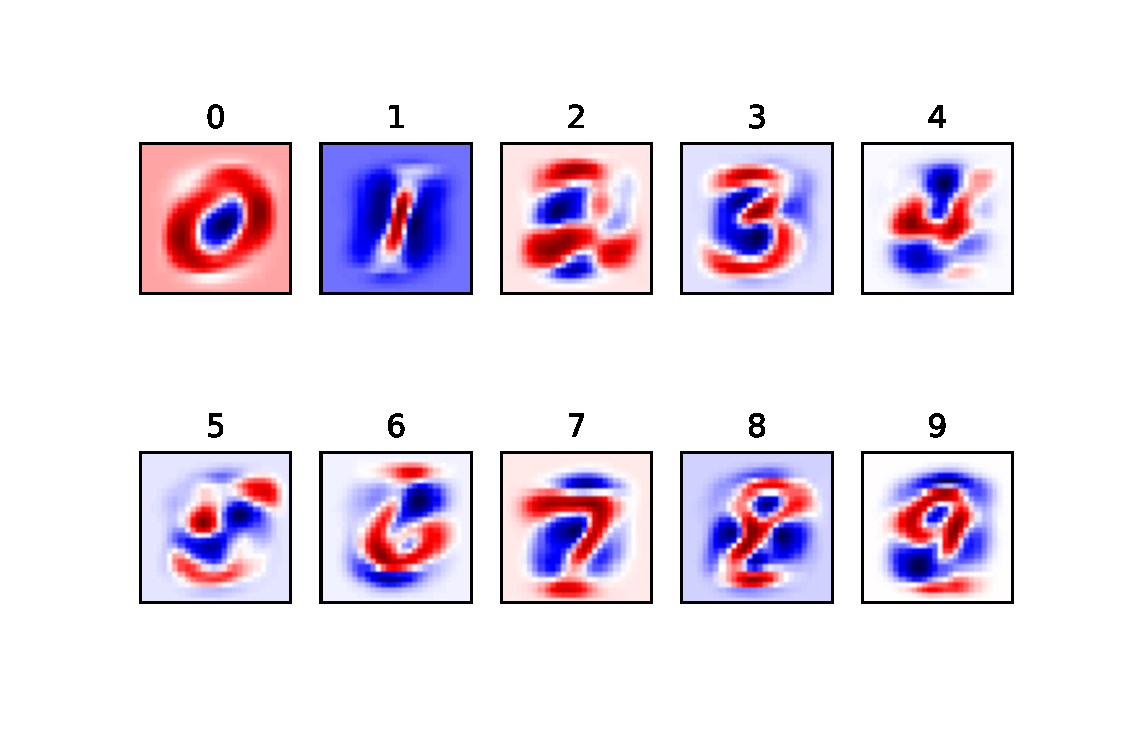
\includegraphics[width=.6\textwidth]{../abbildungen/weightPlot00001.pdf}
	\captionof{figure}{Gewichtungen bei einer Lernrate von 0.0001}
	\label{fig:gewichtung00001}
\end{center}

Wie in Abbildung \ref{fig:gewichtung00001} zu sehen ist, werden bei einer niedrigen Lernrate die Gewichtungen auf die einzelnen Werte so angepasst, dass die Ziffern in den Bildern für den Menschen klar erkenntlich sind. Allerdings ist dieses Vorgehen sehr langsam.

\begin{center}
	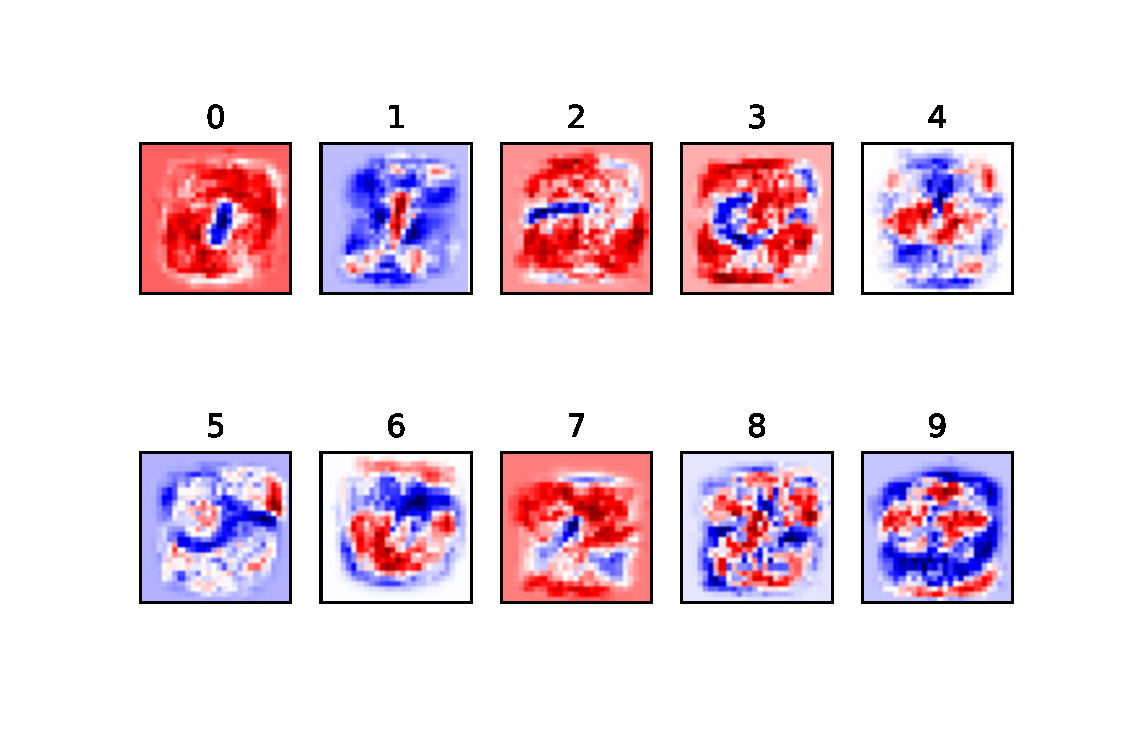
\includegraphics[width=.6\textwidth]{../abbildungen/weightPlot0008.pdf}
	\captionof{figure}{Gewichtungen bei einer Lernrate von 0.008}
	\label{fig:gewichtung0008}
\end{center}

In Abbildung \ref{fig:gewichtung0008} ist eine höhere Lernrate verwendet wurden. Dabei sind die einzelnen Ziffern nicht mehr für den Menschen erkennbar bzw. nur noch zu erraten. Dafür wurde mit dieser Variante eine höhere Genauigkeit erzielt. Generell gilt, je höher die Lernrate ausfällt, desto schlechter sind Ziffern erkennbar.

\section{Probleme}
\label{sec:probleme}
\printsubchapterauthor{\authorNiklas}
Bei der Erstellung des neuronalen Netzes selbst sind keine großen Problem aufgetreten. Die einzigen Probleme, die auftraten fanden bei der Installation statt. Die einfachste Variante der Installation ist über eine virtuelle Umgebung von Anaconda. In dieser virtuellen Umgebung kann TensorFlow installiert werden, ohne die Python-Installation des Rechners zu verändern. Auf einem Mac ist ein relativ neues Betriebssystem nötig, um TensorFlow nutzen zu können. Das Betriesbssystem \textit{El Capitan} reicht dafür nicht aus. Auf einem Ubuntu 18.04 Rechner müssen nach abgeschlossener Installation manche Bibliotheken einzeln installiert werden. Auf einem Windows-Computer werden alle nötigen Bibliotheken bei der Installation mit installiert und TensorFlow ist nach der Installation einsatzbereit.

\chapter{Fazit}
\label{chap:fazit}

%1.Unterkapitel
\section{Vor- und Nachteile von TensorFlow}
\label{sec:vorUndNachteileTensorFlow}
Was ist die Motivation hinter dieser Arbeit

%1.Unterkapitel
\section{Ausblick}
\label{sec:ausblick}
Was ist die Motivation hinter dieser Arbeit

\subsection{TensorFlow Lite}
\label{sec:tensorFlowLite}
Was

% ***************************** BIBLIOGRAPHY **********************************
\baselineskip=14pt
\clearpage
\phantomsection
\addcontentsline{toc}{chapter}{\protect\numberline{}\bibname}
\bibliography{bib/thesis}

% ******************************* APPENDIX ************************************
\appendix
\chapter{Anhang A}
\label{chap:anhang_a}

\subsection{Code des Demonstrators}
\label{sec:codeDemonstrator}
\begin{lstlisting}
from tensorflow.examples.tutorials.mnist import input_data
mnist = input_data.read_data_sets('MNIST_data', one_hot=True)
import matplotlib.pyplot as plt
import numpy as np
import random as ran
%matplotlib inline

import tensorflow as tf

def TRAIN_SIZE(num):
    print ('Total Training Images in Dataset = ' + str(mnist.train.images.shape))
    print ('--------------------------------------------------')
    x_train = mnist.train.images[:num,:]
    print ('x_train Examples Loaded = ' + str(x_train.shape))
    y_train = mnist.train.labels[:num,:]
    print ('y_train Examples Loaded = ' + str(y_train.shape))
    print('')
    return x_train, y_train

def TEST_SIZE(num):
    print ('Total Test Examples in Dataset = ' + str(mnist.test.images.shape))
    print ('--------------------------------------------------')
    x_test = mnist.test.images[:num,:]
    print ('x_test Examples Loaded = ' + str(x_test.shape))
    y_test = mnist.test.labels[:num,:]
    print ('y_test Examples Loaded = ' + str(y_test.shape))
    return x_test, y_test

def display_digit(num):
    print(y_train[num])
    label = y_train[num].argmax(axis=0)
    image = x_train[num].reshape([28,28])
    plt.title('Example: %d  Label: %d' % (num, label))
    plt.imshow(image, cmap=plt.get_cmap('gray_r'))
    plt.show()
        
def display_mult_flat(start, stop):
    images = x_train[start].reshape([1,784])
    for i in range(start+1,stop):
        images = np.concatenate((images, x_train[i].reshape([1,784])))
    plt.imshow(images, cmap=plt.get_cmap('gray_r'))
    plt.show()

x_train, y_train = TRAIN_SIZE(55000)

display_digit(0)

display_mult_flat(0,400)

x = tf.placeholder(tf.float32, shape=[None, 784])
y_ = tf.placeholder(tf.float32, shape=[None, 10])
W = tf.Variable(tf.zeros([784,10]))
b = tf.Variable(tf.zeros([10]))
y = tf.nn.softmax(tf.matmul(x,W) + b)
cross_entropy = tf.reduce_mean(-tf.reduce_sum(y_ * tf.log(y), reduction_indices=[1]))


x_train, y_train = TRAIN_SIZE(5500)
x_test, y_test = TEST_SIZE(10000)
LEARNING_RATE = 0.05
TRAIN_STEPS = 10000

sess = tf.Session()
init = tf.initialize_all_variables()
sess.run(init)

training = tf.train.GradientDescentOptimizer(LEARNING_RATE).minimize(cross_entropy)
correct_prediction = tf.equal(tf.argmax(y,1), tf.argmax(y_,1))
accuracy = tf.reduce_mean(tf.cast(correct_prediction, tf.float32))

for i in range(TRAIN_STEPS+1):
    sess.run(training, feed_dict={x: x_train, y_: y_train})
    if i%100 == 0:
        print('Training Step:' + str(i) + '  Accuracy =  ' + str(sess.run(accuracy, feed_dict={x: x_test, y_: y_test})) + '  Loss = ' + str(sess.run(cross_entropy, {x: x_train, y_: y_train})))
    
for i in range(10):
    plt.subplot(2, 5, i+1)
    weight = sess.run(W)[:,i]
    plt.title(i)
    plt.imshow(weight.reshape([28,28]), cmap=plt.get_cmap('seismic'))
    frame1 = plt.gca()
    frame1.axes.get_xaxis().set_visible(False)
    frame1.axes.get_yaxis().set_visible(False) 
plt.show()


x_train, y_train = TRAIN_SIZE(1) 
display_digit(0)

answer = sess.run(y, feed_dict={x: x_train})
print(answer)

answer.argmax()

def display_compare(num):
    # THIS WILL LOAD ONE TRAINING EXAMPLE
    x_train = mnist.train.images[num,:].reshape(1,784)
    y_train = mnist.train.labels[num,:]
    
    # THIS GETS OUR LABEL AS A INTEGER
    label = y_train.argmax()
    
    # THIS GETS OUR PREDICATION AS A INTEGER
    prediction = sess.run(y, feed_dict={x: x_train}).argmax() 
    
    plt.title('Prediction: %d Label: %d' % (prediction, label))
    plt.imshow(x_train.reshape([28,28]), cmap=plt.get_cmap('gray_r'))
    plt.show()

display_compare(ran.randint(0, 55000))
\end{lstlisting}


\subsection{Code des Beispielgraphen}
\label{sec:codeBeispielGraph}
\begin{lstlisting}
import tensorflow as tf
import numpy as np

#Initialisieren der Variablen
a = tf.Variable(3.0, name = "Variable_a")
b = tf.Variable(4.0, name = "Variable_b")
c = tf.Variable(1.0, name = "Variable_c")
d = tf.Variable(2.0, name = "Variable_d")

x_1 = tf.multiply(a, b, "Multiplikation")
x_2 = tf.add(c, d, "Addieren")
x_3 = tf.substract(x_1, x_2, "Substrahieren")
result = tf.sqrt(x_3, "Wurzel")

with tf.Session() as sess:
	tf.global_variables_initializer()
	sess.run(init)
	res = sess.run(result)
	print("Ergebnis der Berechnung des Graphen:" , res)
\end{lstlisting}

% ***************************** BACK MATTER ***********************************
%\thispagestyle{empty}

%\addcontentsline{toc}{chapter}{\protect\numberline{}Eidesstattliche Erklärung}
%\chapter*{}
\vspace*{0.5cm}
\noindent

Hiermit versichere ich, dass ich die vorliegende Arbeit selbstständig verfasst und keine anderen als die angegebenen Quellen und Hilfsmittel benutzt habe. Ich versichere, dass ich alle wörtlich oder sinngemäß aus anderen Werken übernommenen Aussagen als solche gekennzeichnet habe, und dass die eingereichte Arbeit weder vollständig noch in wesentlichen Teilen Gegenstand eines anderen Prüfungsverfahrens gewesen ist.

\vspace{3cm}
\toponym, den \today

\end{document}